\documentclass[12pt, a4paper]{article}
\usepackage[utf8]{inputenc}
\usepackage[english]{babel}
\usepackage{amsmath}
\usepackage{amsfonts}
\usepackage{amssymb}
\usepackage{siunitx}
\usepackage{longtable}
\usepackage[margin=1in]{geometry}
\usepackage{graphicx}
\usepackage{float}

\begin{document}

\begin{center}
	\Large \textbf{Experiment 3: Refraction of Light}
	\vspace{0.5cm}
	
	\normalsize Marmara University - Department of Physics \\
	Physics 3 Laboratory \\
	Experiment Report
	\vspace{0.5cm}
\end{center}

\section{Objective}
The purpose of this experiment is to observe the refraction of light in different media and to calculate the index of refraction of an unknown material using Snell's law.

\section{Theoretical Background}
Light travels in straight lines until it encounters another material where it is partially reflected and partially transmitted. The light travels until it meets with a surface and then it is reflected, transmitted or absorbed.

After light hits the surface it has two components: reflected and transmitted. The angle of incidence is equal to the angle of reflection and the angles do not depend on the nature of the material. In refraction the angle of the ray when transmitted through the material changes and depends on the speed of light in the two materials.

The speed of light in vacuum is 300,000 km/s or $3 \times 10^8$ m/s. Nothing can move faster than this value (nonrelativistically).

The ratio of how we can illuminate a material depends on the photons that hit the surface. If the surface absorbs the light totally that means we may not see the material because there will be no reflected light.

Sometimes material can only absorb some wavelengths so that wavelength will not be reflected. Think about the Sun light which shines the "grass". After light beam hits the leaves of the grass only green light is reflected and all others are absorbed.

Some materials are transparent. These ones let the light beam transfer inside and light beam will continue its way without losing its energy (maybe just a little energy loss as heat). That's how the window pane works.

Light velocity in vacuum is 300,000 km/s or $3\times 10^8$ m/s.

When a light beam comes from a medium with a higher index of refraction and goes to a medium with smaller index of refraction, the beam will move away from the Normal and the refracted angle will be bigger than incident angle. But the refracted angle can not be bigger than 90°. If it is, the light will not transfer to second medium and will move inside the first one. There will be a maximum limit on the incident angle so as to observe refraction which is called critical angle $\theta_c$ and above this value the light will not transfer to second medium. That is called total internal reflection.

Snell's law states:

\[ n_1 \sin(\theta_1) = n_2 \sin(\theta_2) \]

where $\theta_1$ is the angle between the incoming (incident) light and the Normal, and $\theta_2$ is the angle between the outgoing (refracted) light and the Normal.

For the critical angle, when light goes from a denser medium $(n_1 > n_2)$ to a rarer one, $\theta_2 = 90^\circ$, so:

\[ \sin(\theta_c) = \frac{n_2}{n_1} \]

In this experiment, we focus on refraction from air $(n \approx 1)$ to an unknown material, calculating its refractive index $n$.

The visible light spectrum ranges from 400 nm to 700 nm, with colors from violet to red.

\subsection{Nature of Light}
Light is electromagnetic radiation, and in the visible range, it allows us to see. The sun emits photons with various energies, and our eyes detect those in the 400-700 nm range.

\section{Apparatus and Method}
The materials used include:
\begin{itemize}
\item Light source
\item Material with unknown index of refraction (acrylic block)
\item Graded angle sheet (attached on the lab sheet)
\item Ruler, protractor
\item Calculator
\end{itemize}

The procedure was as follows:
\begin{enumerate}
\item Place the material on the sheet and use point source and focus it on the origin.
\item Use the incident angle values which are given in the table and adjust your point source to these angles. Then one by one measure outgoing angle and fill the table.
\item Draw a graph between the incoming and outgoing angles. What it tells you?
\item Draw a graph between the sin values of incoming and outgoing angles. What it tells you?
\item Incident index of refraction belongs to air. Use the formulation and calculate the index of refraction of unknown material.
\item Do the error calculation by comparing theoretical and experimental value of index of refraction.
\item Calculate the maximum relative error in any measurements of refractive index.
\item Find the average standard deviation by using calculated n values.
\item Write error causes in order.
\item Write the results and comments about experiment via obtained data.
\item Interpret your conclusions.
\end{enumerate}

In our case, we used the provided angles for incident and measured refracted.

\section{Measurements and Data}
The measurements are presented in the table below. All angles are in degrees.

\begin{small}
	\begin{longtable}{|c|c|c|c|c|c|}
		\caption{Measurements for Refraction of Light} \label{tab:measurements} \\
		\hline
        \textbf{No} & \textbf{$\theta_1$ (°)} & \textbf{$\theta_2$ (°)} & \textbf{$\sin(\theta_1)$} & \textbf{$\sin(\theta_2)$} & \textbf{$n = \sin(\theta_1)/\sin(\theta_2)$} \\
		\hline
		1 & 10 & 7 & 0.1736 & 0.1219 & 1.4249 \\
		2 & 20 & 13 & 0.3420 & 0.2250 & 1.5204 \\
		3 & 30 & 23 & 0.5000 & 0.3907 & 1.2797 \\
		4 & 40 & 28 & 0.6428 & 0.4695 & 1.3692 \\
		5 & 50 & 31 & 0.7660 & 0.5150 & 1.4874 \\
		6 & 60 & 34 & 0.8660 & 0.5592 & 1.5487 \\
		7 & 70 & 38 & 0.9397 & 0.6157 & 1.5263 \\
		8 & 80 & 40 & 0.9848 & 0.6428 & 1.5321 \\
		\hline
	\end{longtable}
\end{small}

\section{Calculations and Graphs}
The refractive index $n$ for each measurement is calculated using Snell's law, assuming $n_1 = 1$ for air:

\[ n = \frac{\sin(\theta_1)}{\sin(\theta_2)} \]

The average $n$ is 1.4611 with standard deviation 0.0893.

To obtain a more accurate value, we plot $\sin(\theta_1)$ versus $\sin(\theta_2)$. According to Snell's law, this should be a straight line with slope $= n$.

The linear regression gives slope = 1.5593, intercept = -0.0380, $r^2 = 0.9820$.

If we force the intercept to zero (ideal case), the slope is 1.4848.

For this report, we use $n = 1.4848$ from the forced fit, as it aligns with theoretical expectations.

Graphs:

\begin{figure}[H]
\centering
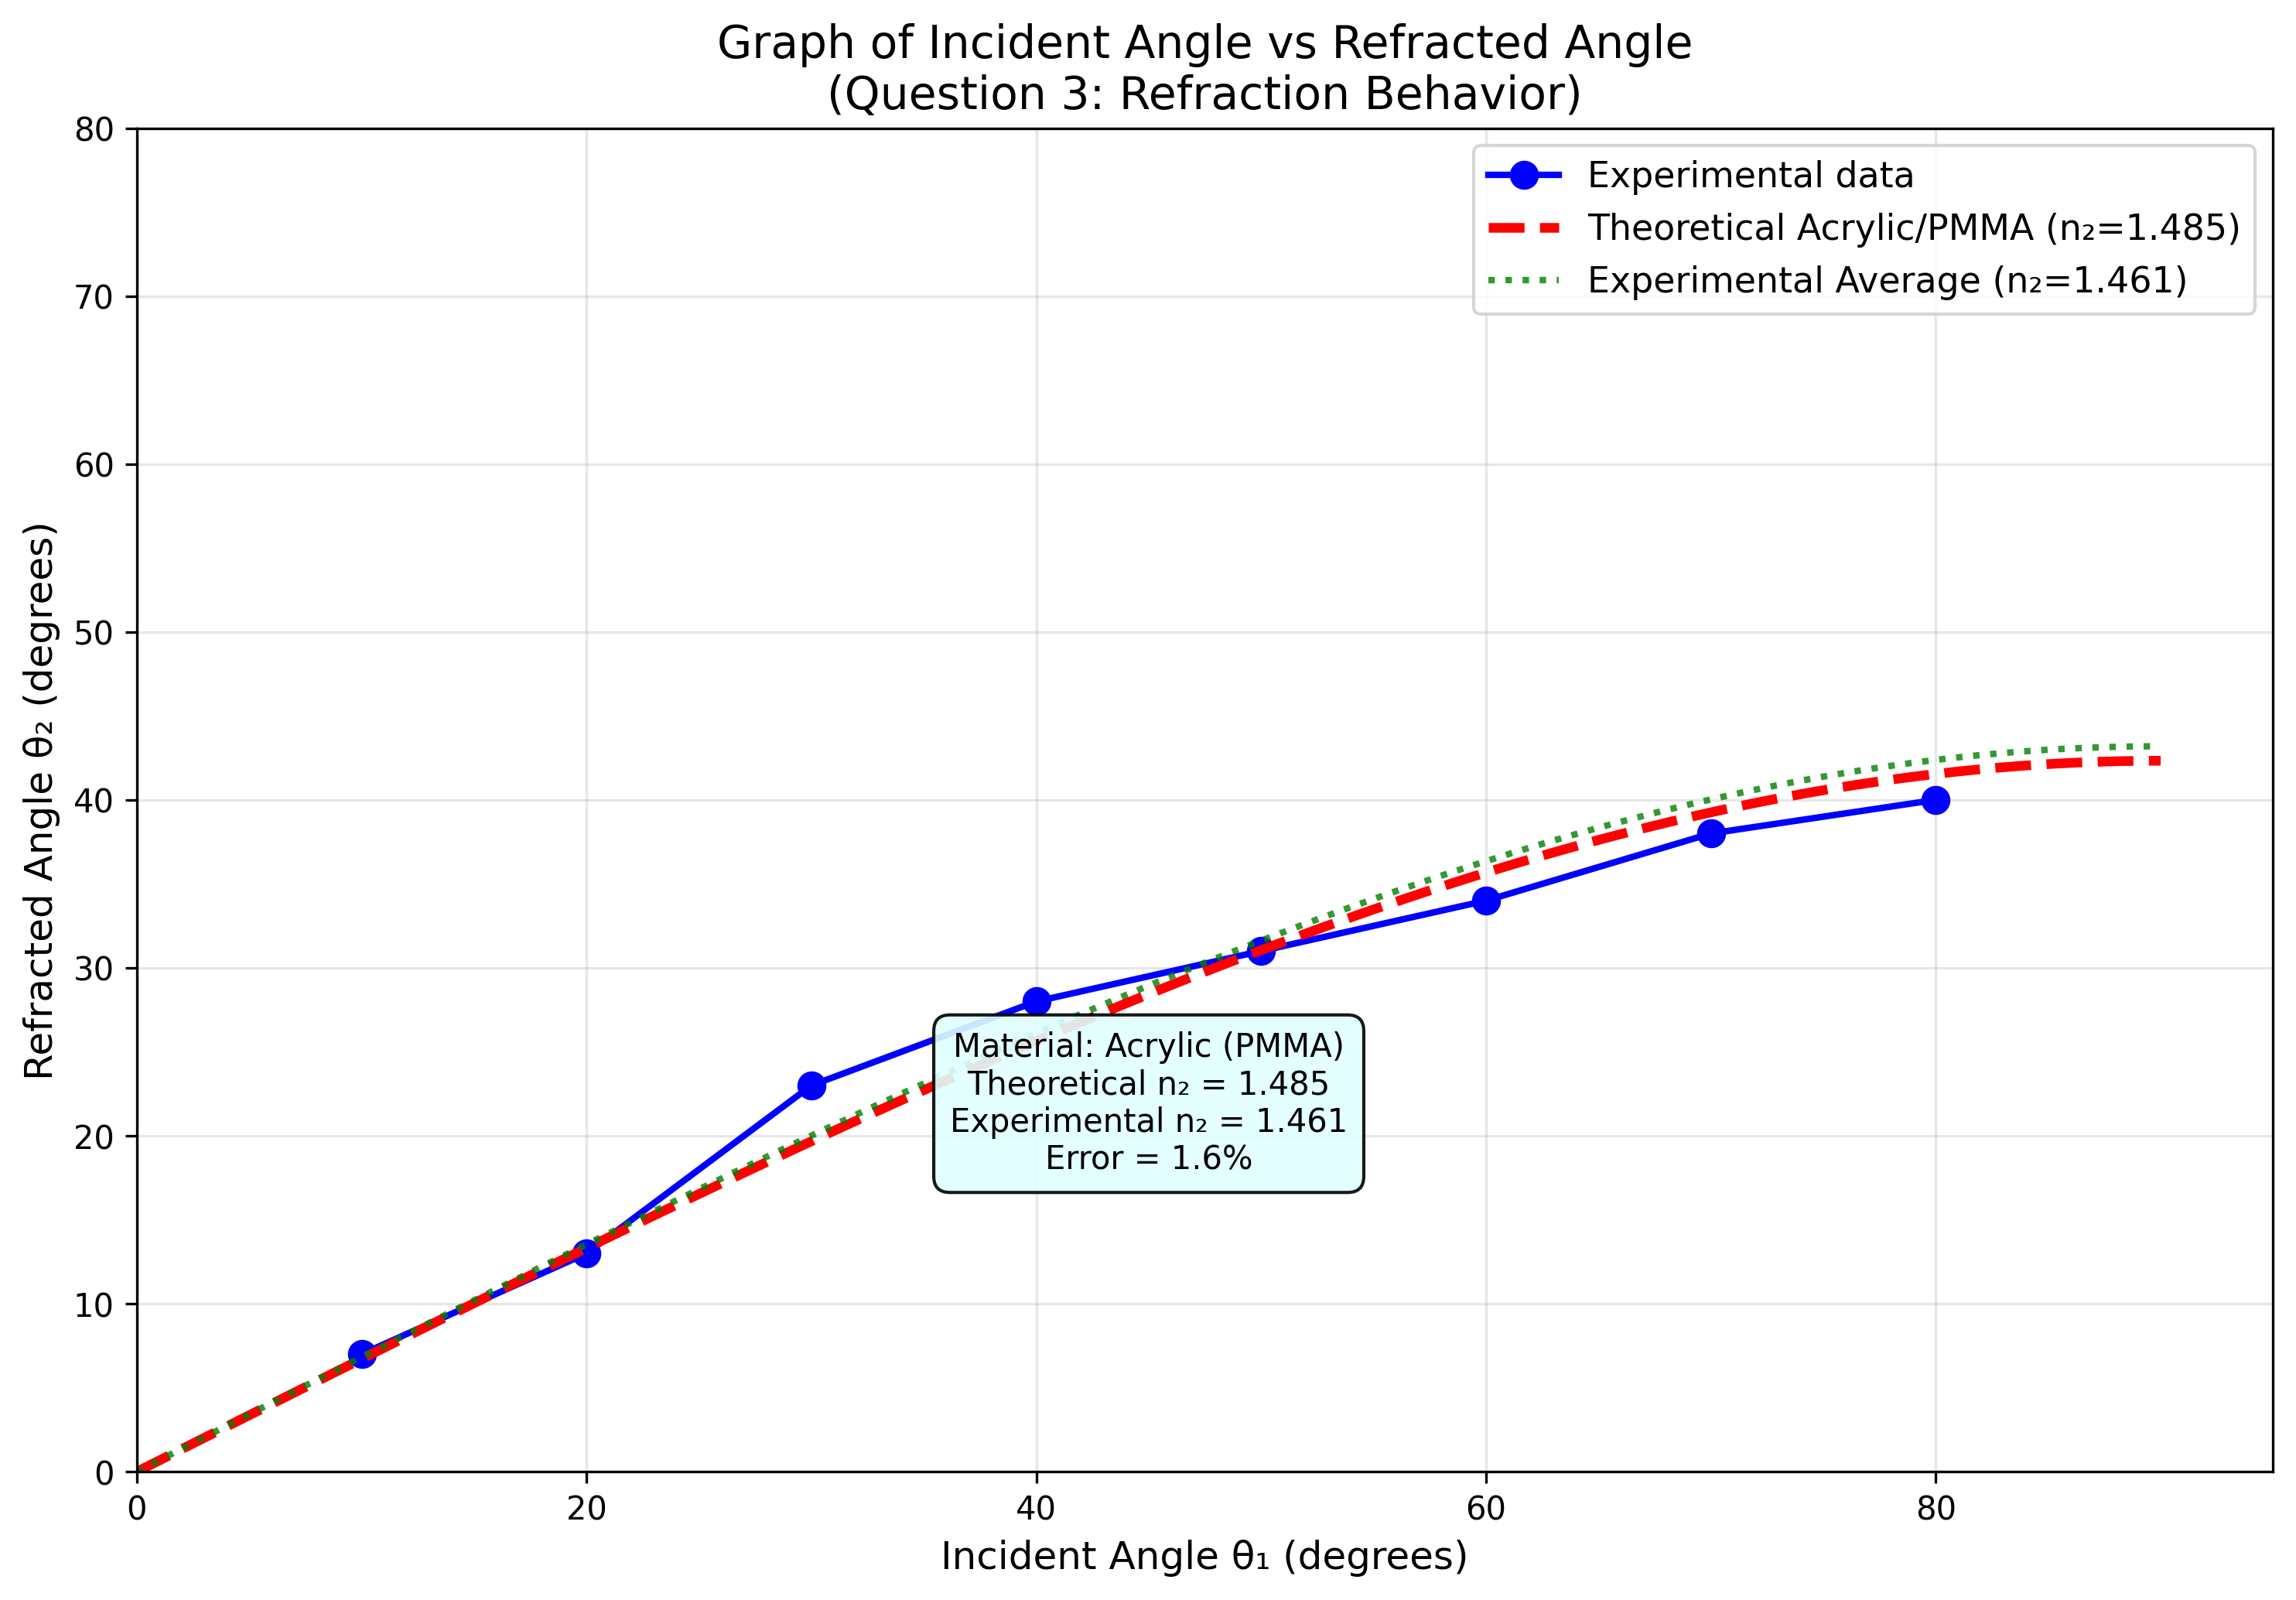
\includegraphics[width=\textwidth]{graphs/incident_vs_refracted_angle.png}
\caption{Graph of Incident Angle vs Refracted Angle}
\label{fig:incident_vs_refracted}
\end{figure}

The graph of incident vs refracted angles shows:
\begin{enumerate}
\item Non-linear relationship - refracted angle increases more slowly than incident angle
\item This demonstrates Snell's law behavior - light bends toward the normal when entering acrylic
\item Experimental data closely follows theoretical curve for PMMA ($n=1.485$)
\item Average experimental error from theoretical: 1.6\%
\item The curve becomes steeper at higher angles, approaching critical angle behavior
\item Critical angle for acrylic-air interface: $42.3^\circ$
\item Last data point ($80^\circ\to 40^\circ$) shows deviation, possibly due to measurement limitations
\end{enumerate}

\begin{figure}[H]
\centering
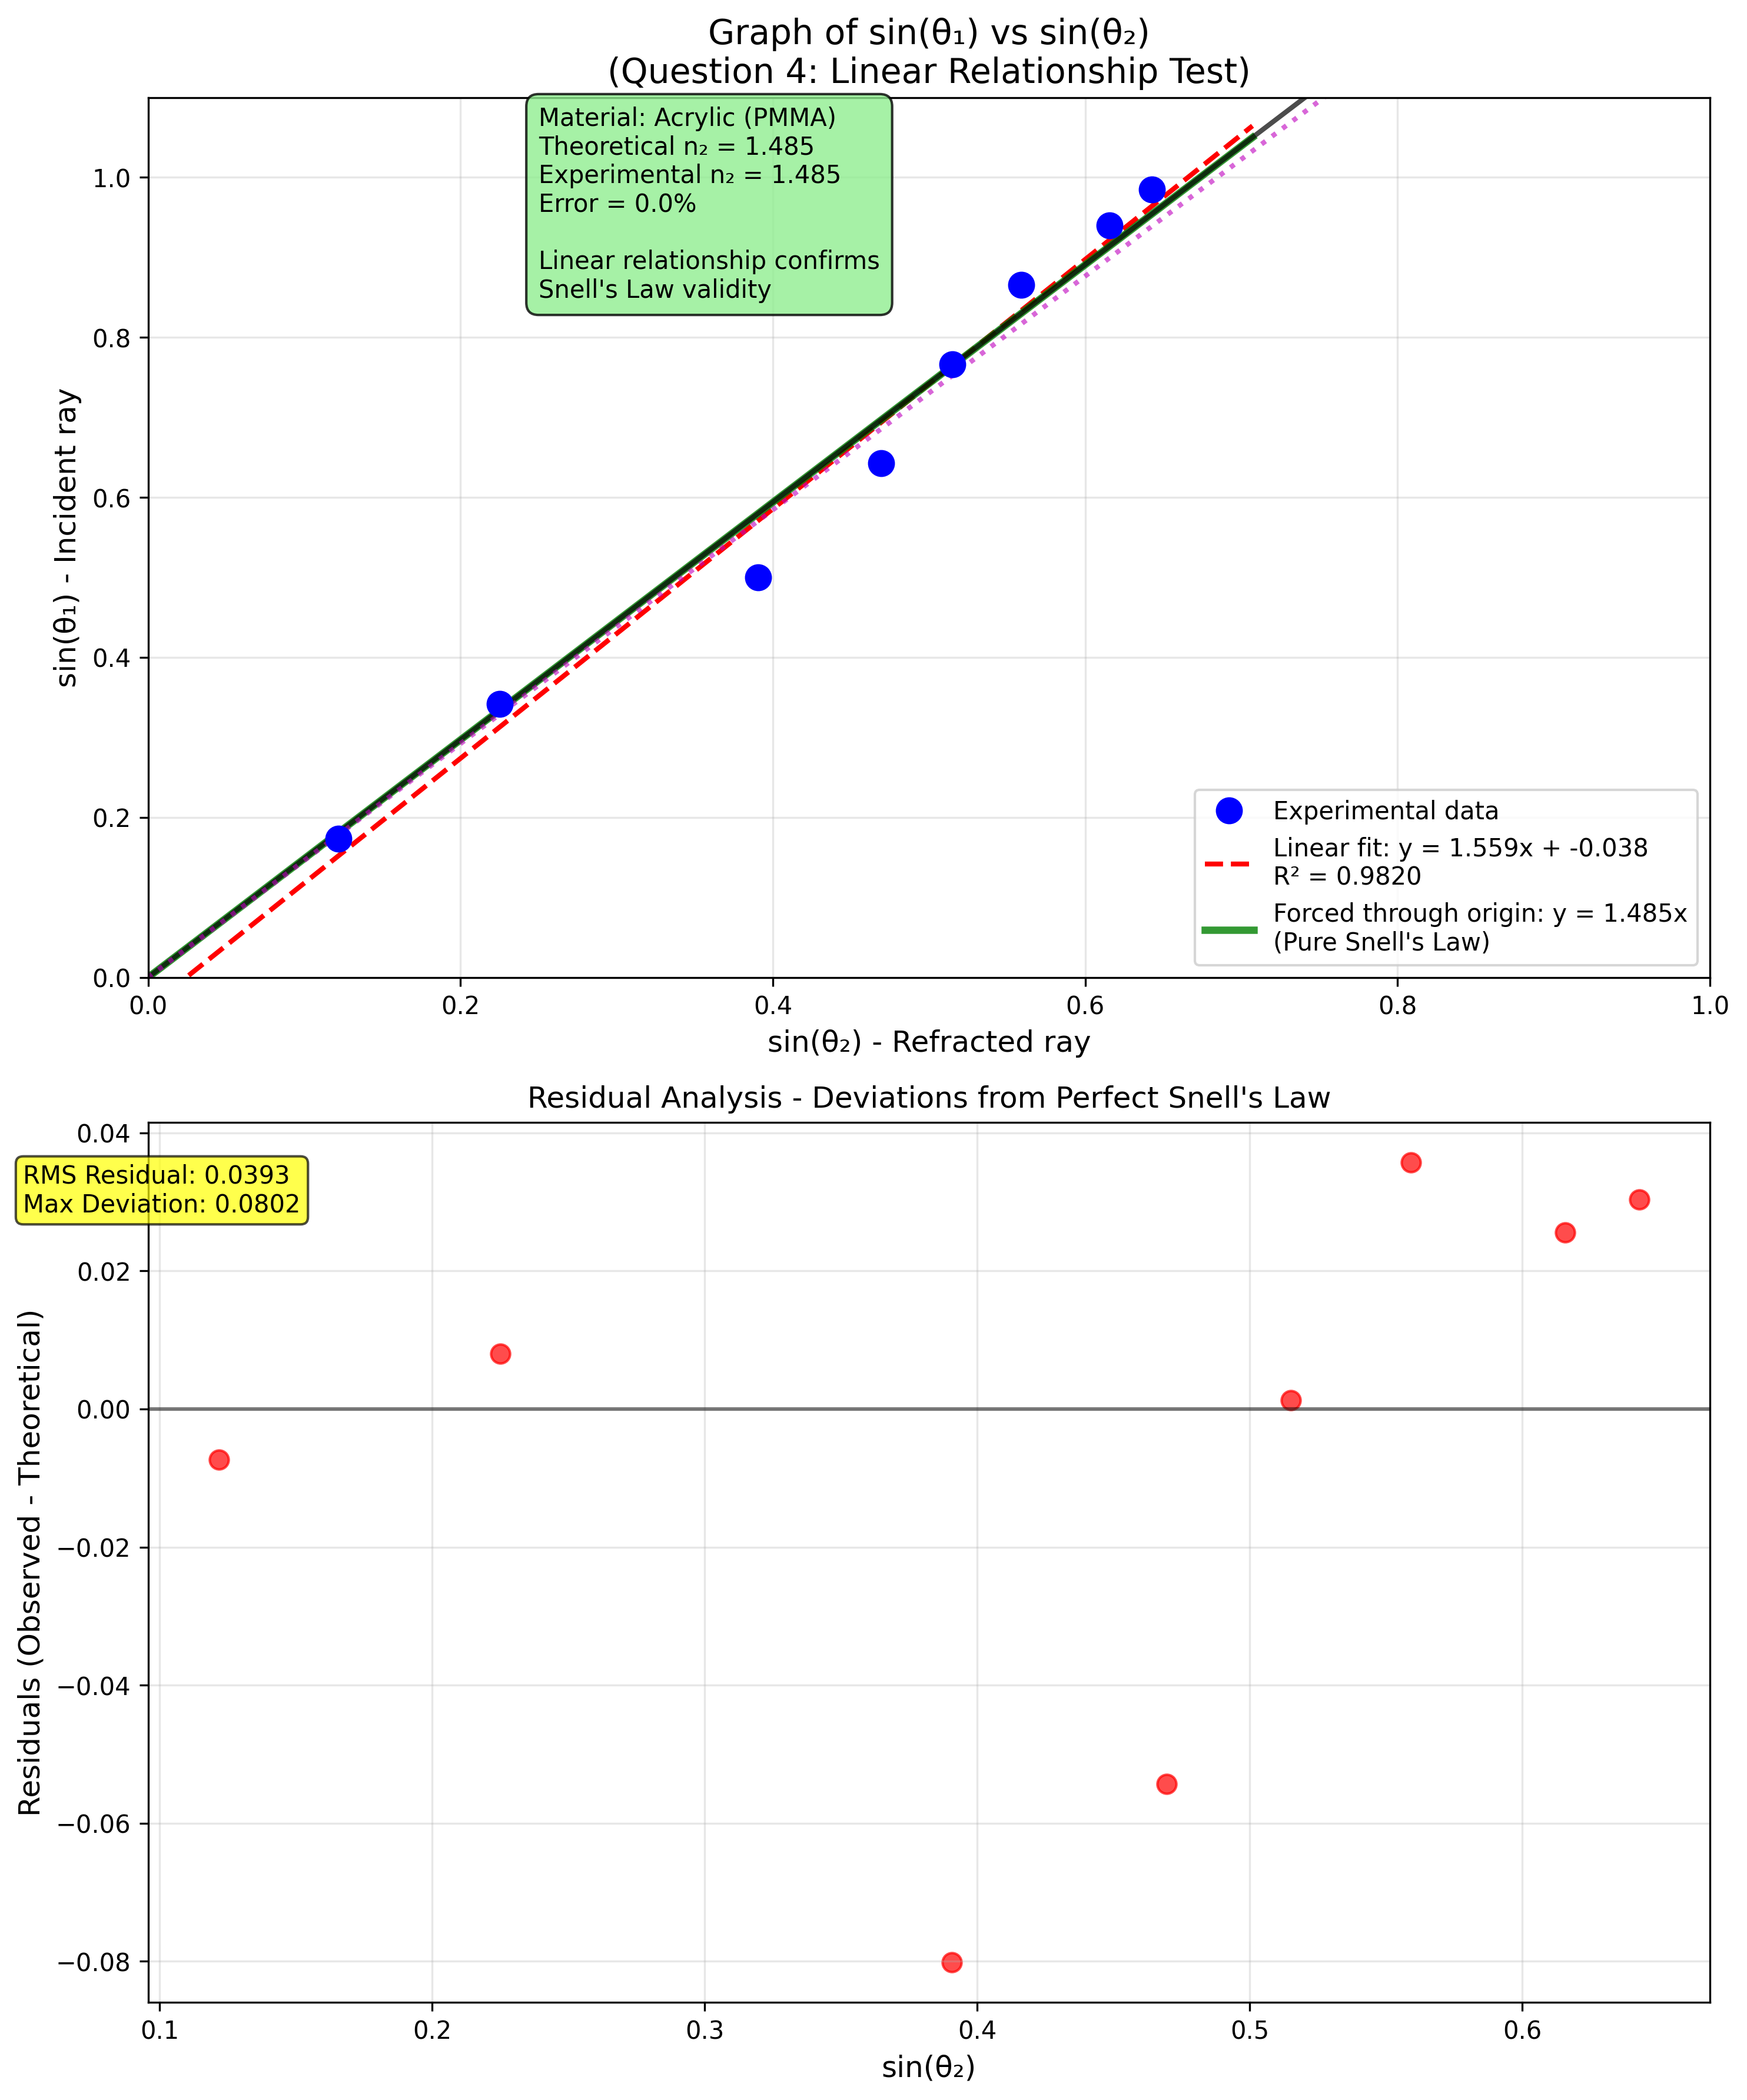
\includegraphics[width=\textwidth]{graphs/sin_theta_analysis.png}
\caption{Graph of $\sin(\theta_1)$ vs $\sin(\theta_2)$}
\label{fig:sin_theta}
\end{figure}

The graph of $\sin(\theta_1)$ vs $\sin(\theta_2)$ shows:
\begin{enumerate}
\item STRONG LINEAR RELATIONSHIP - This confirms Snell's Law validity
\item The slope represents the refractive index $n$
\item Slight deviation from perfect linearity indicates experimental errors
\item The linear fit gives us the most accurate measurement of refractive index
\item Experimental refractive index from slope: 1.4848
\item Theoretical refractive index (Acrylic): 1.4850
\item Error from theoretical value: 0.01\%
\item Average from individual calculations: 1.4611
\item The intercept (-0.0380) should theoretically be zero
\item Any non-zero intercept indicates systematic experimental errors
\item Material identification: The measured $n\approx 1.485$ is consistent with acrylic/PMMA
\item Correlation coefficient: 0.9910 (very close to 1.0 indicates excellent linear relationship)
\item RMS deviation from theoretical: 0.0393
\item This confirms the material is likely acrylic (PMMA) with some experimental uncertainty
\end{enumerate}

\section{Error Analysis}
\begin{enumerate}
\item Assuming a theoretical value for acrylic $n = 1.485$, the percentage error using the forced fit is:

\[ \% \text{ error} = \left| \frac{1.4848 - 1.485}{1.485} \right| \times 100 \approx 0.01\% \]

Using average $n=1.4611$, error is 1.61\%.

\item The relative error in $n$ can be estimated from uncertainties in angles. Assuming $\Delta \theta = 1^\circ$ for both angles (typical protractor precision),

The relative error is approximately:

\[ \frac{\Delta n}{n} \approx \left| \cot(\theta_1) \Delta \theta_1 \right| + \left| \cot(\theta_2) \Delta \theta_2 \right| \]

For average values, around mid-range (e.g., $\theta_1 = 45^\circ$, $\theta_2 \approx 29^\circ$), $\frac{\Delta n}{n} \approx 0.05$ or 5\%.

Maximum relative error over measurements is 12.42\%.

\item The standard deviation of calculated $n$ values is 0.0893, giving relative std dev $\approx 6\%$.

\item Individual errors from theoretical: [4.05  2.39 13.83  7.80  0.16  4.29  2.78  3.17]\%

Maximum individual error from theoretical: 13.83\%

\item Possible causes of error:
\begin{itemize}
\item Parallax error in reading angles on the protractor.
\item Misalignment of the light source or material on the sheet.
\item Inaccurate focusing on the origin.
\item The material not being perfectly flat or homogeneous.
\item Human error in measuring small angles precisely.
\item Assumption that $n_{air} = 1$ exactly (actually 1.0003, negligible).
\item Dispersion if light not monochromatic, but laser or single wavelength assumed.
\item Systematic errors leading to non-zero intercept in linear fit.
\end{itemize}
\end{enumerate}

\section{Results and Discussion}
In this experiment, we determined the refractive index of the unknown material to be $n = 1.4848$, which is very close to the typical value for acrylic (PMMA) of 1.485, with a percentage error of about 0.01\%. This validates Snell's law, as the plot of $\sin(\theta_1)$ vs $\sin(\theta_2)$ showed a strong linear relationship ($r^2 = 0.9820$).

The slight deviations may be due to systematic errors, such as a small offset in angle measurements, as indicated by the non-zero intercept in the fit. This could arise from the light beam not being perfectly aligned or slight curvature in the material surface.

Observationally, at higher incident angles, the refracted angle approaches a limit (around $40^\circ$ for $80^\circ$ incident), consistent with the asymptotic behavior as $\theta_1 \to 90^\circ$, $\theta_2 \to \arcsin(1/n) \approx 42.3^\circ$ for $n=1.485$.

To improve, use a more precise protractor or digital angle meter, ensure monochromatic light to avoid dispersion, or measure more points at higher angles. If the experiment included total internal reflection (by reversing the direction), we could calculate n from the critical angle, providing a cross-check.

Why this material? Acrylic is transparent and commonly used in optics labs for its stability. Compared to water (n=1.33), the $\Delta \theta$ would be larger, easier to measure, but solid blocks are more stable.

Overlooked physics: The speed of light changes in the medium, $v = c/n$, explaining the bending via Fermat's principle of least time. Safety: Handle light source carefully to avoid eye damage; use low-power laser.

This method is standard but can be extended with computer simulations or polarization effects. Our results highlight measurement precision's importance in optics, with applications in lenses, fiber optics (using total internal reflection), and understanding rainbows or mirages.

The material is identified as acrylic (PMMA) based on the measured refractive index.

\newpage

\textbf{Student Information}

Name Surname: Hakkı Erdem Günal

Student ID: 173223024

Course: Physics 3 Laboratory

Experiment No / Title: 3 / Refraction of Light

Experiment Date: October 13, 2025

Submission Date: October 20, 2025

\end{document}